\chapter{Embedded System Architecture}
\label{chap:8}
\newacronym{imu}{IMU}{Inertial Measurement Unit}
In this chapter electronics architecture along with communication scheme is briefly explained. Complete close loop SGCMG unit is realised. Each individual SGCMG unit consist of a three phase close loop brushless motor driver to control reaction wheel at specified angular velocity with given angular acceleration signal. Gimbal motor is driven with Stepper Motor Driver and a dedicated micro-controller which provides appropriate signal to both motor drivers. Angular velocity of gimbal motor is measured using magnetic encoder. Communication protocol is implemented such that each SGCMG unit has dedicated address and returns angular velocity of reaction wheel, angle and angular velocity of gimbal motor when input desired states are provided. Body states of platform such as attitude quaternions, angular rates are computed from 3 axis IMU with dedicated on board master micro-controller for platform. Entire testbed architecture is divided in following major subsystems:
\begin{itemize}
    \item Platform Master State Feedback System
    \item Close Loop SGCMGs
    \item Electrical Power Systems
    \item Ground Control Station Server
\end{itemize}
\section{Platform Master State Feedback System}
Heart of testbench is master micro-controller has primary objective to evaluates platform orientation, body rates from an IMU and communicate in real time with Ground Control Station Server. It can also interact with other SGCMG units if VSCMG control is to be performed on board the platform.
\subsection{Microcontroller}
ESP32 an ultra low power MCU with integrated WiFi by Espressif Systems is used due to it's high performance dual core Tensilica Xtensa LX6 microprocessor running at 160 or 240 MHz, 39 GPIO and supports all standard embedded communication protocols such as 18 Analog-to-Digital Converter (ADC) channels, SPI, UART, I2C PWM output channels, Digital-to-Analog Converters (DAC) I2S interfaces etc, and requires very low power specifically 5V ~100mA(Max). \cite{web:ds_esp32}

\subsection{IMU}
Bosch Sensortech's BNO055 shown in \autoref{fig:BNO} is 9 axis absolute orientation sensor is System in Package includes 3 axis 14-bit accelerometer, 3 axis magnetometer and 3 axis 16-bit gyroscope  and 32-bit microcontroller running on board sensor fusion algorithm.\cite{web:ds_BNO055}
\newacronym{mcu}{MCU}{Microcontroller Unit}
\newacronym{sda}{SDA}{Serial Data}
\newacronym{scl}{SCL}{Serial Clock}
\newacronym{pcb}{PCB}{Printed Circuit Board}
\noindent A custom  \acrshort{pcb} is designed in order to make sure proper and rigid placement of IMU and its interface with microcontroller. Schematic and PCB is shown in \autoref{fig:intefeceIMU} I2C protocol is used to communicate between \acrfull{mcu} and BNO055. \acrshort{sda} and \acrshort{scl} of BNO is connected to GPIO21 and GPIO22 of \acrshort{mcu}. Firmware inside \acrshort{mcu} is programmed in order to update and evaluate current angular velocity and orientation quaternions using Sebastian Madgwick's sensor fusion algorithm \cite{madgwick2010efficient} and send states to Ground station at the speed of 100 Samples per seconds (100Hz).

\begin{figure}[ht]
    \centering
    \begin{subfigure}[b]{0.4\textwidth}
         \centering
         \includegraphics[width=\textwidth]{figures/Electronics/intefeceSCH.pdf}
         \caption{Schematic diagram}
         \label{fig:intefeceSCH}
     \end{subfigure}
    \begin{subfigure}[b]{0.4\textwidth}
         \centering
         \includegraphics[width=\textwidth]{figures/Electronics/intefecePCB.pdf}
         \caption{Printed Circuit Board}
         \label{fig:intefecePCB}
     \end{subfigure}
    \caption{IMU interface board customized for BNO055 and ESP32. }
    \label{fig:intefeceIMU}
\end{figure}

\begin{figure}[ht]
    \centering
    \includegraphics[width=0.35\textwidth]{figures/Assembly/bno055.pdf}
    \caption{BNO055 Absolute orientation sensor consist of triaxial accelerometer, triaxial gyroscope and triaxial magnetometer with on-board 32bit MCU running sensor fusion algorithm}
    \label{fig:BNO}
\end{figure}

\section{Close Loop SGCMG}
Close loop SGCMG module consist of a brushless motor as reaction wheel and stepper motor to drive gimbal. Three phase brushless motor is controlled using commercial of the shelf low cost Electric Speed Controller. ESCs are sensor less speed controllers and use back EMF to estimate rotor position in order to generate step sequence so that proper coils are energised for required angular velocity. Only drawback of sensor less ESC is, it has very high dead band that is due to the fact that at lower speed back EMF is very small hence ESC can not estimate its rotor position. 20A ESC shown in \autoref{fig:esc} is used for this thesis. It has integrated SILABS EFM8BB21F16 MCU ruining at 48MHz, and N channel MOSFETs. BLHELI S open source firmware inside MCU allows bidirectional rotation of motor. It requires 50Hz PWM signal with pulse width varying from 1ms to 2ms. Firmware is configured such a way that motor is at rest at 1.5ms pulse width, max angular velocity at 2ms in clockwise direction and max angular velocity in counterclockwise direction at 1ms. It has very small form factor,with particular dimensions of $23.5\times12\times4mm^3$ and weighs only 6g.
\begin{figure}[ht]
    \centering
    \includegraphics[width=0.5\textwidth]{figures/Assembly/ESC.pdf}
    \caption{20 A Sensorless Electronic Speed Controller}
    \label{fig:esc}
\end{figure}

\noindent Gimbal (NEMA17 Stepper) motor should be driven with special sequence of energizing coils to advance step by step in desired direction. Polulu stepper motor shield shown in \autoref{fig:drv8825} is used to control the gimbal. This shield is based on Texas Instruments DRV8825 microstepping bipolar stepper motor driver it has adjustable current limiting, over-current and over-temperature protection, and six micro stepping resolutions (up to 1/32-step). It operates from 8.2 V to 45 V and current up to 1.5A per phase.
\begin{figure}[ht]
    \centering
    \includegraphics[width=0.5\textwidth]{figures/Assembly/drv8825.pdf}
    \caption{Polulu DRV8825 stepper motor driver shield}
    \label{fig:drv8825}
\end{figure}

\noindent Since stepper motor works in terms of incremental steps, there is possibility that microcontroller may miss few steps, moreover every time MCU is powerd on it does not have exact angular position of stepper motor. For this reason and to have estimate of gimbal angle and angular velocity. AS5600 shown in \autoref{fig:as5600} is a 12-bit on-axis magnetic rotary position sensor is used. This contact less sensor provides analog, PWM and I2C interface. It measures absolute angle from radially magnetized on-axis magnet placed on shaft. 
\begin{figure}[ht]
    \centering
    \includegraphics[width=0.5\textwidth]{figures/Assembly/AS5600.pdf}
    \caption{AS5600 magnetic encoder with radially magnetized magnet of 5mm diameter}
    \label{fig:as5600}
\end{figure}

\noindent Each \acrshort{sgcmg} unit is equipped with a dedicated \acrshort{mcu}. ESP8266 D1 Mini is selected for it's small form factor precisely $34.2\times25.6\times7 mm^3$ and weighs only $8.2g$ is powerful mini WiFi enabled board  with 4MB flash based on ESP-8266EX running at 80/160MHz. It has 11 digital IO, interrupt,pwm,I2C,one-wire interface one analog input and a micro USB port to upload firmware. WiFi compatibility allows complete wireless control and monitoring of SGCMG unit in real time. Complete schematic of SGCMG unit is shown in \autoref{fig:sch_sgcmg_wiring}. Principle function of \acrshort{mcu} is as follows:
\begin{itemize}
    \item Measure angular position of gimbal using AS5600 over I2C.
    \item Control Gimbal motor to achieve desired angle and angular velocity as commanded.
    \item Generate appropriate PWM for ESC to accelerate BLDC at desired angular velocity.
    \item Communicate with server and report current state of gimbal angle, angular velocity and BLDC angular velocity.
\end{itemize}

\begin{figure}[ht]
    \centering
    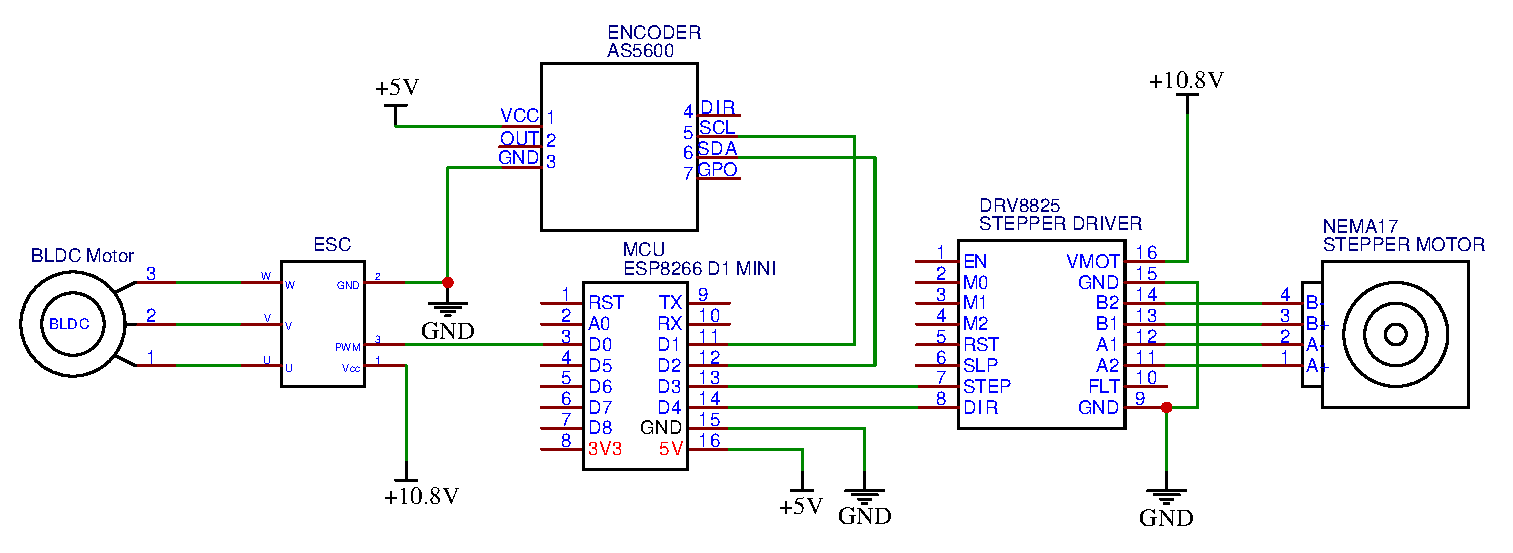
\includegraphics[width=\textwidth]{figures/Assembly/sgcmg_wiring.pdf}
    \caption{Schematic diagram of Close loop SGCMG electronics and wiring}
    \label{fig:sch_sgcmg_wiring}
\end{figure}

\section{Electrical Power System}
Considering power requirement of different components available on platform, pack of Lithium-ion batteries is used as main power source for the complete platform.Samsung's cylindrical Li-ion cell in standard  ICR18650-26F form factor has nominal voltage 3.7V with 2.6Ah energy storage capacity moreover it can provide continuous current up to 5A and weighs 47.0 grams. Since we are using 900KV (900 RPM/V) brushless motor, with the intention of achieving required maximum angular velocity three Li-Ion cells are arranged in series accumulating total output of $11.1V$. A standard 3 cell case is used to hold pack of 3 Li-ion batteries. A dedicated low cost battery management system is attached the battery pack as per \autoref{fig:sch_BMS}. Total weight of battery pack including BMS and case shown in \autoref{fig:BAT18650} sums up to 170 grams. Four units of these battery packs are connected in parallel. Along with 20A total output current capacity, reason for selecting four battery packs is to evenly distribute mass about yaw axis and keeping symmetry of design. 
\begin{figure}[ht]
    \centering
    \includegraphics[width=0.6\textwidth]{figures/Assembly/BMS.pdf}
    \caption{Schematic diagram of 11.1V 5A Battery Management System with 18650 Li-Ion batteries in series}
    \label{fig:sch_BMS}
\end{figure}

\begin{figure}[ht]
    \centering
    \includegraphics[width=0.6\textwidth]{figures/Assembly/BAT18650Case.pdf}
    \caption{Rendered view of Case with three Li-Ion Batteries connected in series to make 3S Li-Ion battery pack}
    \label{fig:BAT18650}
\end{figure}

\noindent 3A DC to DC step down converter shown in \autoref{fig:sch_smps} is used to convert 11.1V to 5V required by AS5400 and \acrshort{mcu}. MP1584EN is a high frequency step-down switching regulator with an integrated internal high-side high voltage power MOSFET. Complete Electrical Power System schematic of VSCMG shown in \autoref{fig:sch_EPS} contains 4 battery packs connected in parallel has 11.1V output supplied to all the SGCMG units. 5V required by \acrshort{mcu}, sensors and motor drivers is provided through two MP1584EN step down converters. This type of modular design simplified the build process since only one unit is to be made and tested and it is easy to replicate same systems with reduced cost. It also reduced debugging complexity since faulty unit can easily be separated and tested individually.

\begin{figure}[ht]
    \centering
    \includegraphics[width=0.5\textwidth]{figures/Assembly/buckConvertor.pdf}
    \caption{MP1584EN 3A DC to DC step down converter configured to convert 11.1V to 5.0V}
    \label{fig:sch_smps}
\end{figure}

\begin{figure}[ht]
    \centering
    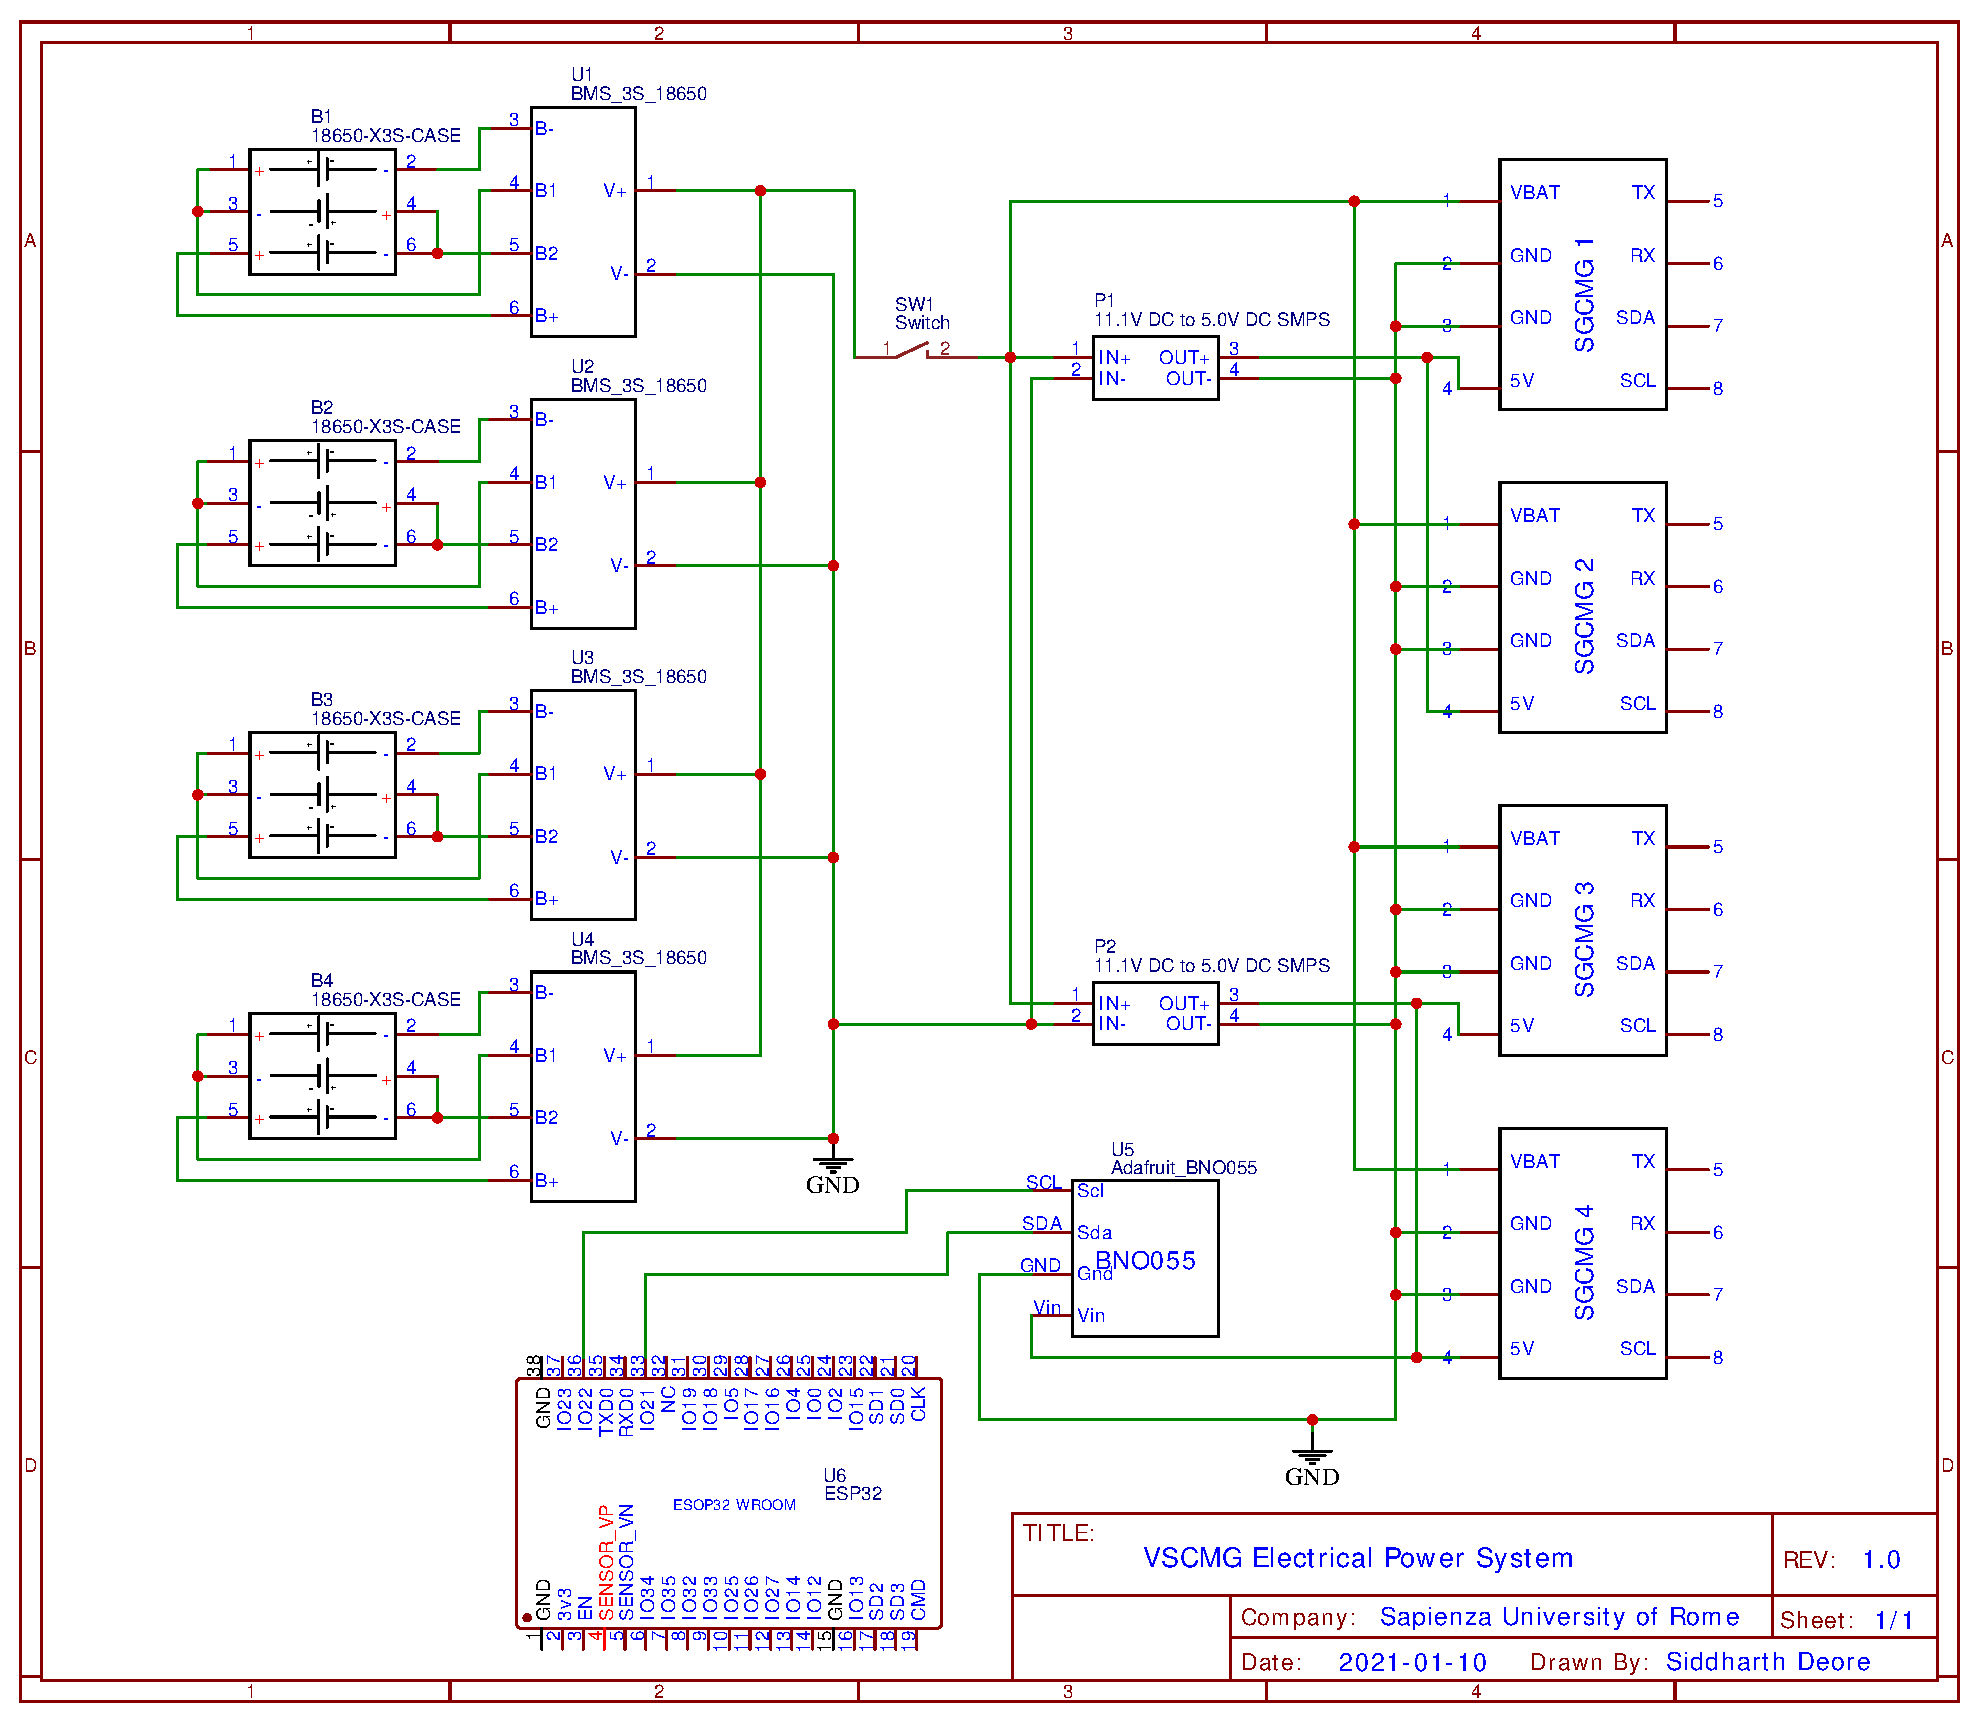
\includegraphics[width=\textwidth]{figures/Assembly/EPS.pdf}
    \caption{Wiring schematic of complete VSCMG test bed Electrical Power System}
    \label{fig:sch_EPS}
\end{figure}
\newacronym{udp}{UDP}{User Datagram Protocol} 
\section{Ground Control Station Server}
Most important part of \acrshort{vscmg} \acrshort{acs} testbed is its novel ground control station server software. Prime functionalities of VSCMG command, control and telemetry architecture are receive platform state such as body rate and attitude quaternions as well as state of each individual SGCMG unit which includes angular velocity of reaction wheel, gimbal angle and gimbal angular velocity. Afterwords, compute the signals to be provided to actuators based on selected  control and steering algorithm and send command signal to each SGCMG unit simultaneously display all the state variables with 3D visualization of entire system. 
\subsection{Communication}
\newacronym{crc}{CRC}{Cyclic Redundancy Check}
Since each SGCMG unit and master platform has its own WiFi enabled \acrshort{mcu}, all the communication requirements are solved using standard network protocol in particular \acrfull{udp} due to simplicity of implementation and fast communication speed with least latency. Ground station server listens on port 3333 over UDP protocol. Each MCU on board as soon as powered on connected to same network SSID of server start transmitting their respective states packaged in specific format to server on same port 3333. As soon as server receives the states from all MCUs it updates all the state variables on GUI simultaneously replies with the command signals for particular MCU. Server communication loop is running at 1000Hz and can easily increased which is far beyond actuator and sensor loop time requirements for this reason even though control and steering law is ported on server computer high speed communication simulates as if control is happening inside on board computer. In this thesis a custom messaging protocol designed on the top of UDP is developed. String of bytes transmitted or received on UDP buffer. There are three different types of message packets. A telemetry payload described in \autoref{tbl:tlm_c2s} is 7 byte packet transmitted from SGCMG to server it contains unique 8bit address of MCU, gimbal angle and reaction wheel angular velocity represented in two bytes each. Last two bytes are \acrfull{crc} computed with buffer starting from byte 0 to byte 4.

\begin{table}[!h]
        \centering
\begin{tabular}{|p{0.1\textwidth}|p{0.2\textwidth}|p{0.6\textwidth}|}
\hline 
 byte & Mnemonic & Description \\
\hline 
 0 & ADDR & Address of MCU \\
\hline 
 1 & GMB\_H & Gimbal Angle high byte \\
\hline 
 2 & GMB\_L & Gimbal Angle low byte \\
\hline 
 3 & OMG\_H & Reaction wheel angular velocity \\
\hline 
 4 & OMG\_L & Reaction wheel angular velocity \\
\hline 
 5 & CRC\_H & CRC hight byte \\
\hline 
 6 & CRC\_L & CRC low byte \\
 \hline
\end{tabular}
        \caption{Telemetry Payload from SGCMG to Server}
        \label{tbl:tlm_c2s}
        \end{table}
\noindent Command packet transmitted to SGCMG shown in \autoref{tbl:tlm_s2c} contains address of destination MCU, 2 byte data of magnetic encoder offset correction, command gimbal angular velocity, and command reaction wheel angular velocity ended with 2 bytes of CRC.
\begin{table}[!h]
        \centering
\begin{tabular}{|p{0.10\textwidth}|p{0.20\textwidth}|p{0.60\textwidth}|}
\hline 
 byte & Mnemonic & Description \\
\hline 
 0 & ADDR & Address of MCU \\
\hline 
 1 & OFFSET\_H & Magnetic Encoder offset high byte \\
\hline 
 2 & OFFSET\_L & Magnetic Encoder offset low byte \\
\hline 
 3 & CMD\_GMB\_H & Command Gimbal Angular velocity high byte \\
\hline 
 4 & CMD\_GMB\_L & Command Gimbal Angular velocity low byte \\
\hline 
 5 & CMD\_OMG\_H & Command RW Angular velocity high byte \\
\hline 
 6 & CMD\_OMG\_L & Command RW Angular velocity low byte \\
\hline 
 7 & CRC\_H & CRC hight byte \\
\hline 
 8 & CRC\_L & CRC low byte \\
 \hline
\end{tabular}
        \caption{Command Payload from Server to SGCMG MCU}
        \label{tbl:tlm_s2c}
        \end{table}
        
\noindent Similarly, 17 byte packet is transmitted from Master to server contains 8 bit address of master, quaternion vector, and body rate vector having two bytes for each element of vector and at last 2 bytes CRC computed with buffer from byte 0 to byte 14 as given in \autoref{tbl:tlm_m2s}

This type of coding scheme allows fast data transmission without conflicting any variable, in addition since data is sent in string made up of chunks of 8 bit (byte), same coding scheme can be ported easily to various embedded communication protocols such as UART or I2C making it easy to port control algorithm on board master controller based on users choice. Note that \acrshort{crc} appended at the end of each message is 16 bit error detecting code following IBM CRC-16 also referred as CRC-16-ANSI X3.28 polynomial representations of cyclic redundancy check with polynomial $x^{16}+x^{15}+x^2+1$.
\begin{table}[!h]
        \centering
        
\begin{tabular}{|p{0.1\textwidth}|p{0.2\textwidth}|p{0.6\textwidth}|}
\hline 
 byte & Mnemonic & Description \\
\hline 
 0 & ADDR & Address of MCU \\
\hline 
 1 & Q0\_H & Quaternion 0 high byte \\
\hline 
 2 & Q0\_L & Quaternion 0 low byte \\
\hline 
 3 & Q1\_H & Quaternion 1 high byte \\
\hline 
 4 & Q1\_L & Quaternion 1 low byte \\
\hline 
 5 & Q2\_H & Quaternion 2 high byte \\
\hline 
 6 & Q2\_L & Quaternion 2 low byte \\
\hline 
 7 & Q3\_H & Quaternion 3 high byte \\
\hline 
 8 & Q3\_L & Quaternion 4 low byte \\
\hline 
 9 & omegaX\_H & Body rate aboute x axis high byte \\
\hline 
 10 & omegaX\_L & Body rate aboute x axis low byte \\
\hline 
 11 & omegaY\_H & Body rate aboute y axis high byte \\
\hline 
 12 & omegaY\_L & Body rate aboute y axis low byte \\
\hline 
 13 & omegaZ\_H & Body rate aboute z axis high byte \\
\hline 
 14 & omegaZ\_L & Body rate aboute z axis low byte \\
\hline 
 15 & CRC\_H & CRC hight byte \\
\hline 
 16 & CRC\_L & CRC low byte \\
 \hline
\end{tabular}
        \caption{Telemetry Payload from Master MCU to Server}
        \label{tbl:tlm_m2s}
        \end{table}

